\documentclass{article}
\usepackage{amsmath}
\usepackage{graphicx}

\title{Problema de Optimización de VRPTW con Extensiones}
\author{Tu Nombre}
\date{}

\begin{document}

\maketitle

\section{Descripción del Problema}

El Problema de Enrutamiento de Vehículos con Ventanas de Tiempo (VRPTW, por sus siglas en inglés) es una extensión del Problema de Enrutamiento de Vehículos (VRP) en el que se deben respetar ventanas de tiempo para la entrega o recogida de mercancías en cada cliente. El objetivo es minimizar el costo total de las rutas, que puede incluir la distancia recorrida, el número de vehículos utilizados, o ambos, mientras se respetan las restricciones de capacidad de los vehículos y las ventanas de tiempo de los clientes.

\section{Modelo Matemático}

\subsection{Parámetros}

\begin{itemize}
    \item \( V = \{0, 1, 2, \dots, n\} \): Conjunto de nodos, donde \( 0 \) es el depósito y \( 1, 2, \dots, n \) son los clientes.
    \item \( K \): Conjunto de vehículos.
    \item \( c_{ij} \): Costo de viajar desde el nodo \( i \) al nodo \( j \).
    \item \( d_i \): Demanda del cliente \( i \).
    \item \( Q_k \): Capacidad del vehículo \( k \).
    \item \( [a_i, b_i] \): Ventana de tiempo del cliente \( i \), donde \( a_i \) es el tiempo más temprano para comenzar el servicio y \( b_i \) es el tiempo más tardío.
    \item \( s_i \): Tiempo de servicio en el cliente \( i \).
    \item \( t_{ij} \): Tiempo de viaje desde el nodo \( i \) al nodo \( j \).
    \item \( M \): Un número suficientemente grande.
    \item \( \alpha \): Penalización por llegar antes de la ventana de tiempo.
    \item \( \beta \): Penalización por llegar después de la ventana de tiempo.
    \item \( f_k \): Consumo de combustible del vehículo \( k \) por unidad de distancia.
    \item \( C_k \): Capacidad de combustible del vehículo \( k \).
\end{itemize}

\subsection{Variables de Decisión}

\begin{itemize}
    \item \( x_{ijk} \): Variable binaria que es 1 si el vehículo \( k \) viaja desde el nodo \( i \) al nodo \( j \), y 0 en caso contrario.
    \item \( w_{ik} \): Tiempo en el que el vehículo \( k \) comienza el servicio en el nodo \( i \).
    \item \( y_{ik} \): Cantidad de carga en el vehículo \( k \) después de visitar el nodo \( i \).
    \item \( z_{ik} \): Cantidad de combustible en el vehículo \( k \) después de visitar el nodo \( i \).
\end{itemize}

\subsection{Función Objetivo}

Minimizar el costo total de las rutas, incluyendo penalizaciones por violaciones de ventanas de tiempo:

\[
\text{Minimizar} \quad Z = \sum_{k \in K} \sum_{i \in V} \sum_{j \in V} c_{ij} x_{ijk} + \alpha \sum_{k \in K} \sum_{i \in V} \max(a_i - w_{ik}, 0) + \beta \sum_{k \in K} \sum_{i \in V} \max(w_{ik} - b_i, 0)
\]

\subsection{Restricciones}

\begin{enumerate}
    \item \textbf{Restricción de visitas únicas}: Cada cliente debe ser visitado exactamente una vez.

    \[
    \sum_{k \in K} \sum_{i \in V} x_{ijk} = 1 \quad \forall j \in V \setminus \{0\}
    \]

    \item \textbf{Restricción de flujo}: Si un vehículo llega a un cliente, debe salir de él.

    \[
    \sum_{i \in V} x_{ihk} - \sum_{j \in V} x_{hjk} = 0 \quad \forall h \in V \setminus \{0\}, \forall k \in K
    \]

    \item \textbf{Restricción de capacidad}: La suma de las demandas de los clientes en una ruta no debe exceder la capacidad del vehículo.

    \[
    y_{ik} + d_j \leq Q_k \quad \forall i, j \in V, \forall k \in K
    \]

    \item \textbf{Restricción de ventana de tiempo}: El tiempo de servicio en cada cliente debe estar dentro de su ventana de tiempo, con penalizaciones.

    \[
    a_i \leq w_{ik} \leq b_i \quad \forall i \in V, \forall k \in K
    \]

    \item \textbf{Restricción de tiempo de viaje}: El tiempo de llegada a un cliente debe ser coherente con el tiempo de salida del cliente anterior más el tiempo de viaje.

    \[
    w_{ik} + s_i + t_{ij} - w_{jk} \leq M (1 - x_{ijk}) \quad \forall i, j \in V, \forall k \in K
    \]

    \item \textbf{Restricción de combustible}: El consumo de combustible no debe exceder la capacidad del tanque.

    \[
    z_{ik} - f_k \cdot c_{ij} \geq 0 \quad \forall i, j \in V, \forall k \in K
    \]

    \item \textbf{Restricción de inicio y fin en el depósito}: Cada vehículo debe comenzar y terminar su ruta en el depósito.

    \[
    \sum_{j \in V} x_{0jk} = 1 \quad \forall k \in K
    \]
    \[
    \sum_{i \in V} x_{i0k} = 1 \quad \forall k \in K
    \]

    \item \textbf{Restricción de recogida y entrega}: Para cada par de recogida y entrega, el vehículo debe visitar el nodo de recogida antes que el nodo de entrega.

    \[
    w_{pk} \leq w_{dk} \quad \forall (p, d) \in \text{Pares de recogida y entrega}, \forall k \in K
    \]
\end{enumerate}

\section{Objetivos Adicionales}

\subsection{Minimizar el Tiempo Total}

\[
\text{Minimizar} \quad T = \sum_{k \in K} \sum_{i \in V} w_{ik}
\]

\subsection{Balancear Cargas}

\[
\text{Minimizar} \quad B = \sum_{k \in K} \left( \sum_{i \in V} y_{ik} - \frac{\sum_{i \in V} d_i}{|K|} \right)^2
\]

\subsection{Maximizar la Satisfacción del Cliente}

\[
\text{Maximizar} \quad S = -\left( \alpha \sum_{k \in K} \sum_{i \in V} \max(a_i - w_{ik}, 0) + \beta \sum_{k \in K} \sum_{i \in V} \max(w_{ik} - b_i, 0) \right)
\]

\section{Gráficos}

A continuación, se presenta un ejemplo gráfico de una solución al VRPTW con las extensiones propuestas.

\begin{itemize}
    \item El nodo central (0) representa el depósito.
    \item Los nodos periféricos (1, 2, 3, 4) representan los clientes.
    \item Las flechas representan las rutas de los vehículos.
    \item Las etiquetas en los nodos indican la ventana de tiempo de cada cliente.
\end{itemize}

\begin{center}
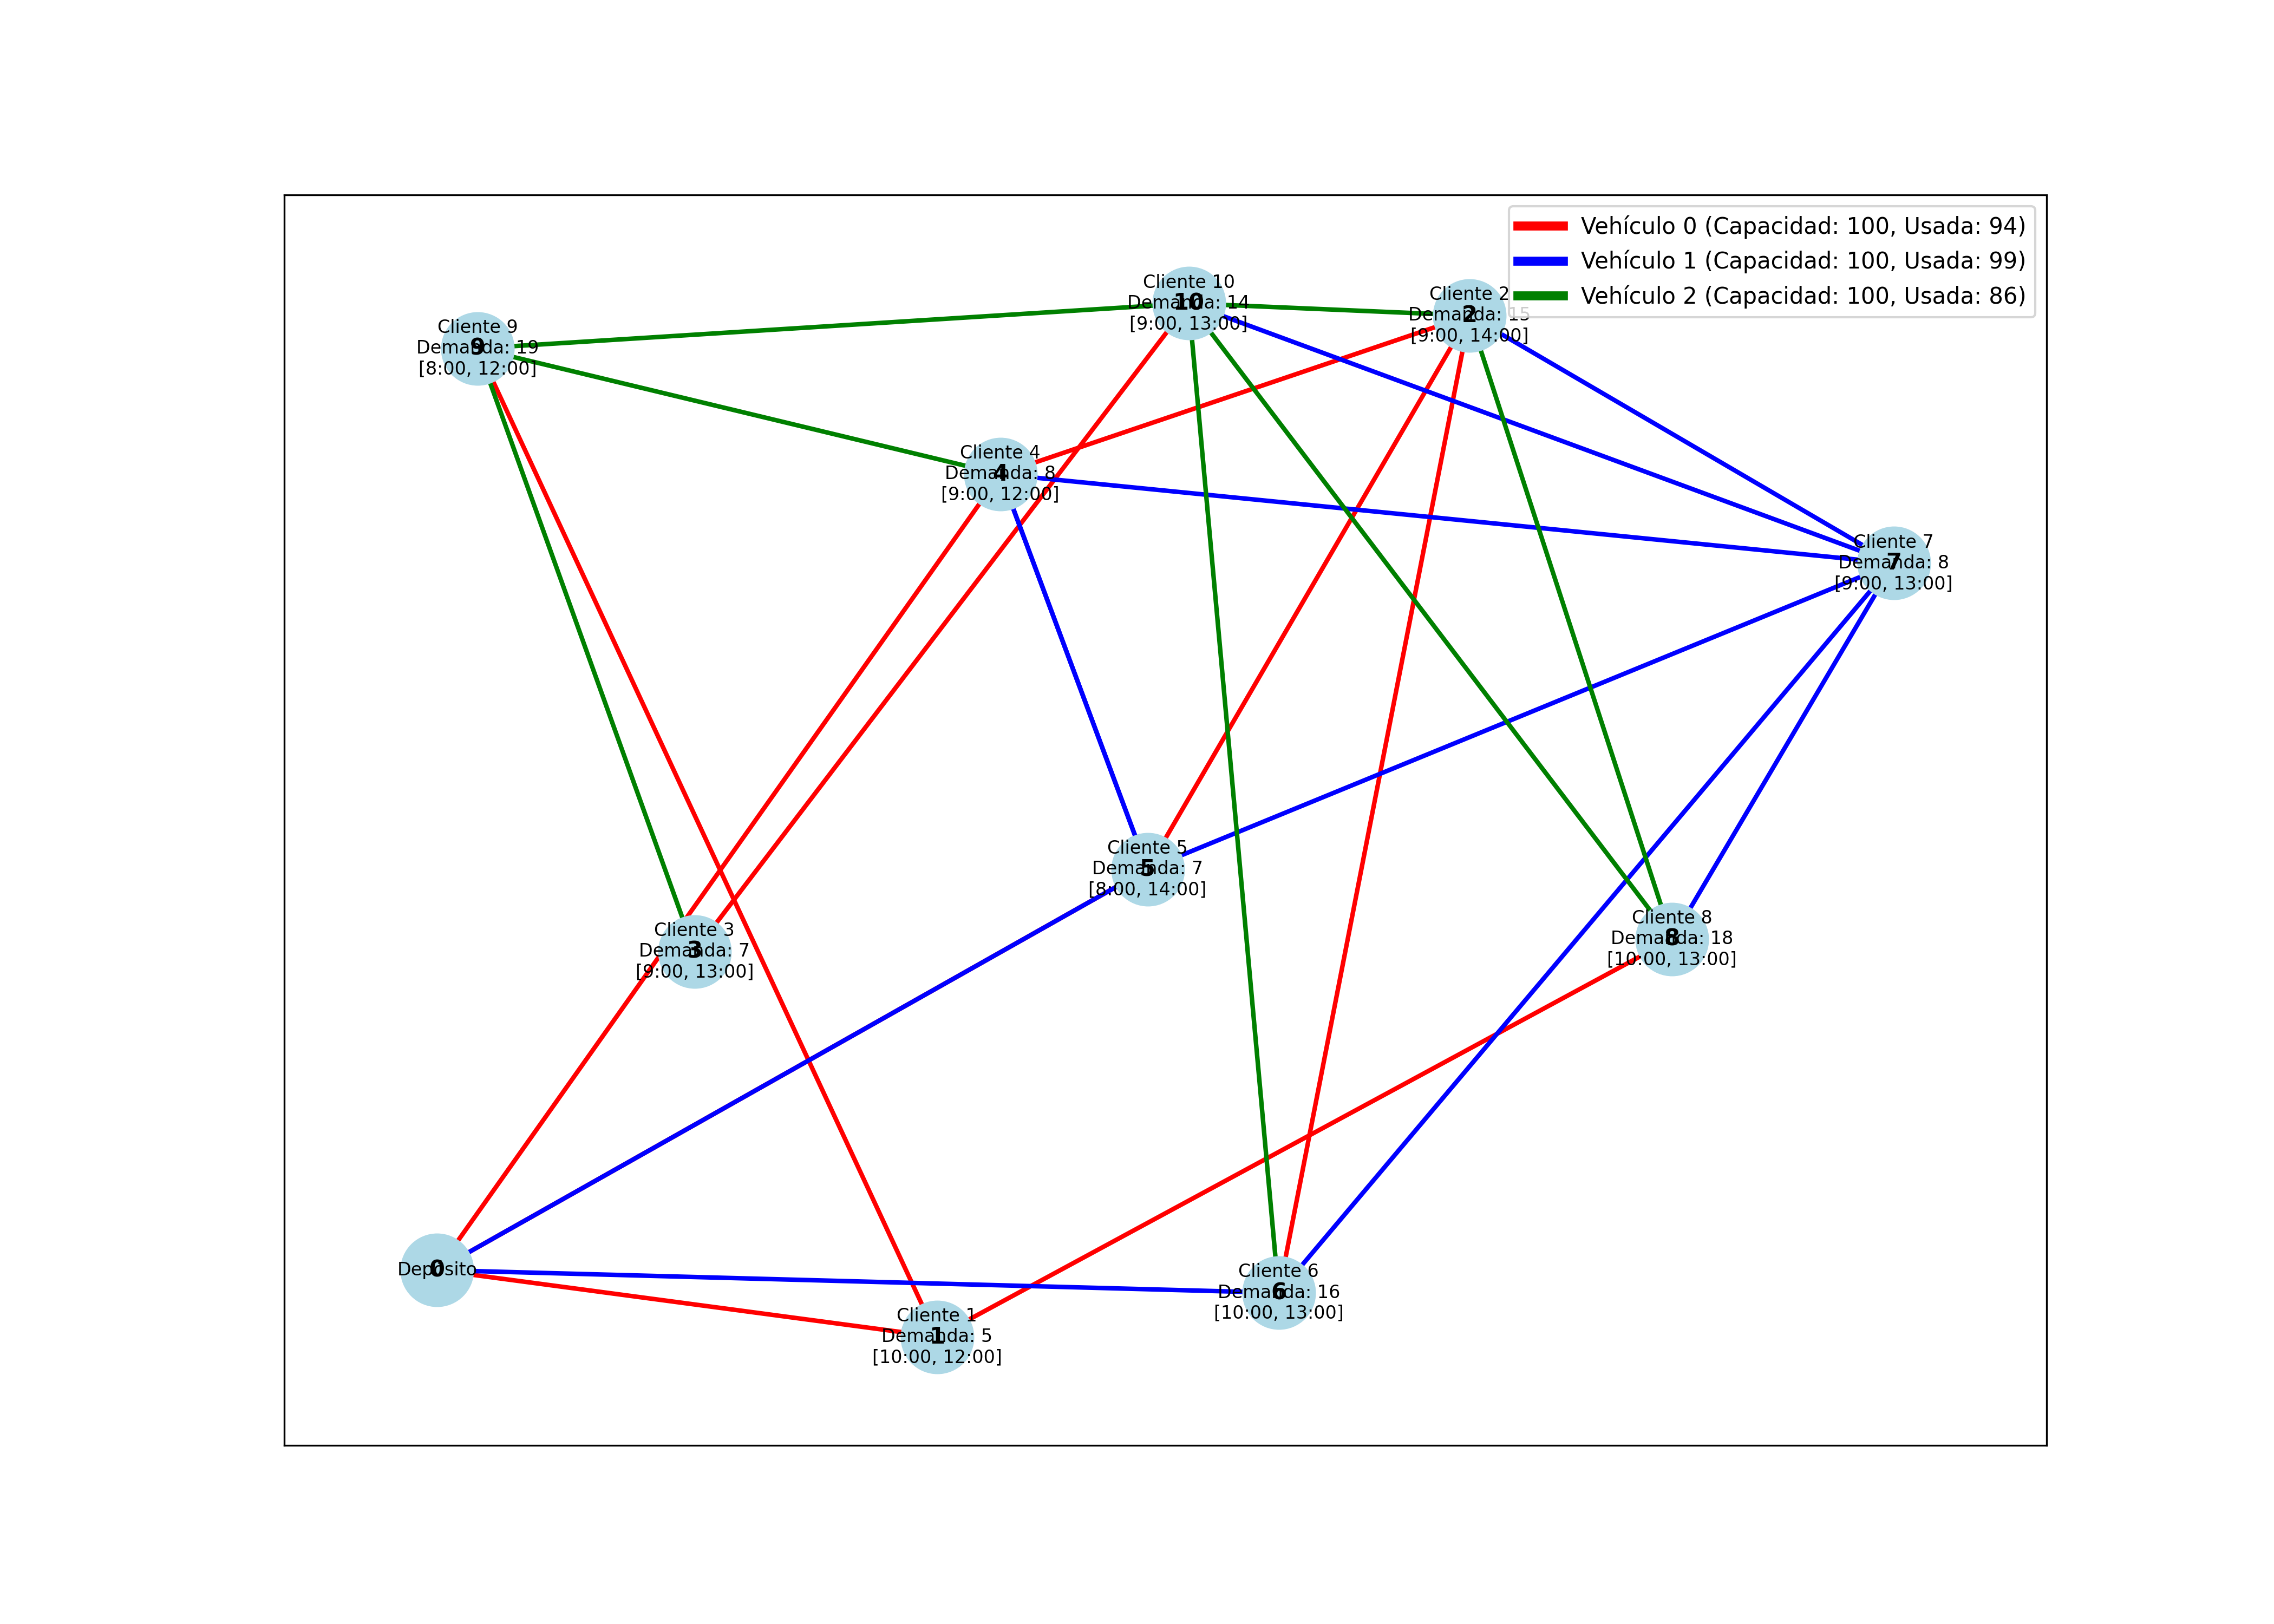
\includegraphics[width=1.0\textwidth]{vrptw_large_graph_with_capacity.png}
\end{center}

\end{document}